\subsection{Esercizio 7}
Utilizzare le $function$ del precedente esercizio per determinare una approssimazione
della radice della funzione
\[
        f(x) = \left[x - cos(\frac{\pi}{2}x)\right]^3,
\]
per $tol = 10^{-3}, 10^{-6}, 10^{-9}, 10^{-12},$ partendo da $x_0 = 1$
(e $x_1 = 0.99$ per il metodo delle secanti). Tabulare i risultati,
in modo da confrontare le iterazioni richieste da ciascun metodo. Commentare
i risultati ottenuti.
\newline \textbf{Soluzione:}

Eseguendo lo script \nameref{cod:7} si ottengono i risultati contenuti nella tabella \ref{tab:7}
e nella figura \ref{fig:es7}. Come si può notare, il metodo di newton e il metodo delle secanti
convergono molto più rapidamente del metodo di bisezione e del metodo delle corde.
\begin{table}[h]
        \renewcommand\arraystretch{2}
        \resizebox{\columnwidth}{!}{
                \begin{tabular}{|l l l l l|}
                        \hline
                        Metodo                &        & newton                & secanti               & steffensen            \\
                        \hline
                        tolleranza$=10^{-3}$  & \vline & 5.969479343078770e-01 & 5.991437227787725e-01 & 5.973965526716639e-01 \\
                        tolleranza$=10^{-6}$  & \vline & 5.946140179818806e-01 & 5.946156634766230e-01 & 5.946143706333854e-01 \\
                        tolleranza$=10^{-9}$  & \vline & 5.946116464662755e-01 & 5.946116487688006e-01 & 5.946130329177074e-01 \\
                        tolleranza$=10^{-12}$ & \vline & 5.946116440592810e-01 & 5.946116440610053e-01 & 5.946130329177074e-01 \\
                        \hline
                \end{tabular}
        }
        \caption{valori approssimati con i metodi di Newton, secanti e Steffensen}
        \label{tab:7}
\end{table}
\begin{figure}[!ht]
        \centering
        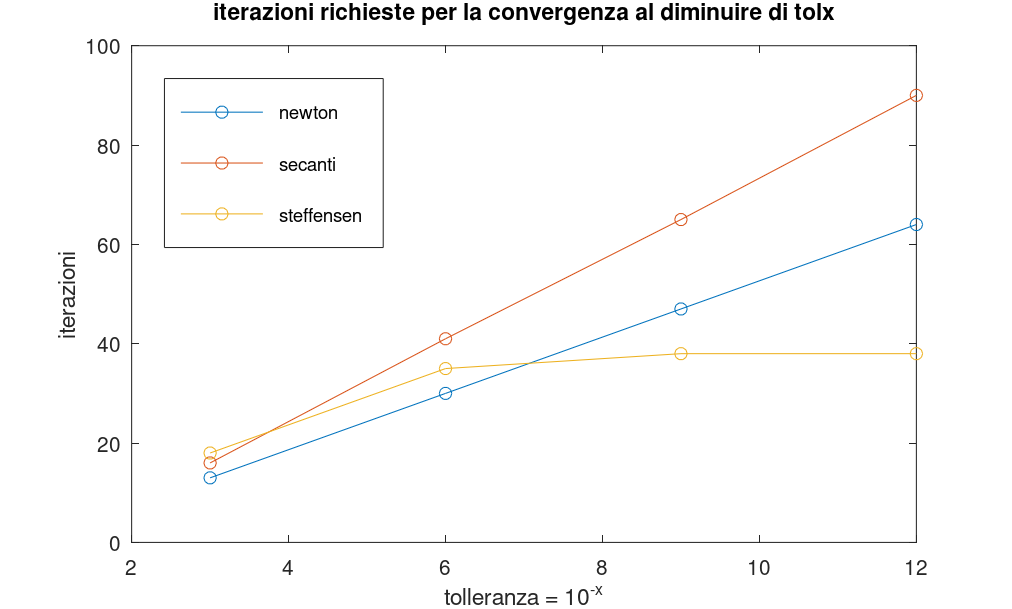
\includegraphics[width=16cm,height=12cm,keepaspectratio]{capitolo2/es7_figure.png}
        \caption{iterazioni richieste}
        \label{fig:es7}
\end{figure}
\FloatBarrier
In iterazione $38$ la funzione con metodo di Steffensen falliscie con valori di tolleranza
$10^-9$ e $10^-12$. Ed infatti, si vede che in questi valori la figura \ref{fig:es7}
rimane costante rispetto iterazioni. Questo fallimento dato da divizione a zero.
\newline \textbf{Costo computazionale} \newline
È possibile valutare i costi computazionali dei algoritmi verificando il numero
di funzioni richiamate all'interno dei codici, mediante feval:
\begin{itemize}
        \item Newton: $2i$, $i=1:maxit$;
        \item Secanti: $1 + i$, $i=1:maxit$;
        \item Steffensen: $2i$, $i=1:maxit$;
\end{itemize}
